\documentclass[12pt, a4paper]{article}
\usepackage{graphicx}
\usepackage[english]{babel}
\usepackage[nottoc]{tocbibind}
\usepackage[ddmmyyyy]{datetime}
\renewcommand{\dateseparator}{.}
\renewcommand{\figurename}{Şekil}
\usepackage{cite}
\bibliographystyle{ieeetr}
\usepackage{pdflscape}
\renewcommand{\refname}{Kaynakça}
%opening

\title{\bf\fontsize{12pt}{14pt}\selectfont KÜTAHYA SAĞLIK BİLİMLERİ ÜNİVERSİTESİ\\MÜHENDİSLİK VE DOĞA BİLİMLERİ FAKÜLTESİ }

\begin{document}
	\maketitle
	\begin{figure}[h]
		\centering
		
\includegraphics{logo}\\ \
		
		 \author{Özge ÇITAKOĞLU} \\
		\date{\today} 
		%\date{\DTMnow}
		%\date{\DTMnow}
	\end{figure}  
	\begin{center}
		\title{\bf\fontsize{12pt}{14pt}\selectfont YAPAY ZEKA RAPORU \\
			Reinforcement Learning Kullanarak Robotun Labirentte Gezinmesi  }
	\end{center}
	\newpage
		
	
	\section{Giriş}
	\begin{itemize}
		\item Günümüzde yapay zeka ve makine öğrenmesi alanındaki gelişmeler, çeşitli problemlere etkili çözümler sunmaktadır. Bu raporda, robotların labirent gibi karmaşık ortamlarda gezinmelerini sağlamak için kullanılan iki önemli algoritma olan A* ve Q-learning ele alınacaktır. A* algoritması, en kısa yolu bulmak için deterministik bir yaklaşım sunarken, Q-learning, deneyime dayalı olarak öğrenme sürecini optimize eden bir pekiştirmeli öğrenme algoritmasıdır. Bu algoritmaların nasıl çalıştığı ve birbirlerine karşı avantajları ile dezavantajları detaylı bir şekilde incelenecektir.
		
\item A* algoritması (A-star), bir graf veya grid üzerinde en kısa veya en maliyet etkin yolu bulmak için kullanılan bir arama algoritmasıdır. Genellikle labirent veya haritalarda yol bulma problemleri için kullanılır. 

\item Q-learning, bir ajanın (örneğin bir oyuncunun) bir ortamda nasıl hareket edeceğini öğrenmesini sağlayan bir pekiştirmeli öğrenme algoritmasıdır. Amaç, ajanın belirli bir durumda en iyi aksiyonu seçerek ödülünü maksimize etmesidir



\item  Farkları: A Algoritması*: Deterministik ve planlama bazlı bir yaklaşımdır. Hedefe ulaşmak için önceden tanımlanmış bir yol bulur. Genellikle statik ve belirli bir çevrede kullanılır.
Q-Learning: Deneyim tabanlı ve öğrenme odaklı bir yaklaşımdır. Ajan, ödüller ve cezalar üzerinden deneyim kazanarak en iyi stratejiyi öğrenir. Dinamik ve değişen çevrelerde kullanılabilir.
Özetle, A* algoritması belirli bir hedefe en kısa yolu bulurken, Q-learning bir ajanı bir ortamda en iyi hareketleri yaparak ödüllerini maksimize etmeyi öğrenmeye yönlendirir. Bu iki teknik, farklı türde problemler için güçlü araçlar sunar.

\item Bu kod, Pygame kullanarak bir labirent oyunu oluşturur. Oyunda bir oyuncu (Q-learning algoritmasını kullanan) ve düşmanlar bulunmaktadır. Oyuncunun amacı, labirentin başlangıç noktasından bitiş noktasına ulaşmaktır.

\item A* Algoritması Heuristic fonksiyonu: İki nokta arasındaki Manhattan mesafesini hesaplar.
A fonksiyonu*: Başlangıç (start) ve bitiş (end) noktaları arasındaki en kısa yolu bulur. Q-Learning Oyuncusu
QLearningPlayer sınıfı: Oyuncu karakterini temsil eder.
init metodu: Oyuncunun başlangıç konumu, sağlık durumu ve Q-learning parametreleri (öğrenme oranı, indirim faktörü, keşif oranı) ayarlanır.
update metodu: Oyuncunun güncellenmesini sağlar. Q-learning algoritması ile hareket eder ve ödül hesaplamalarını yapar.
get reward metodu: Oyuncunun belirli bir duruma (konuma) geldiğinde alacağı ödülü hesaplar.


\end{itemize}
\begin{landscape}
	\begin{figure}[!ht]	
		
			\caption[]{}
		\centering 
		
		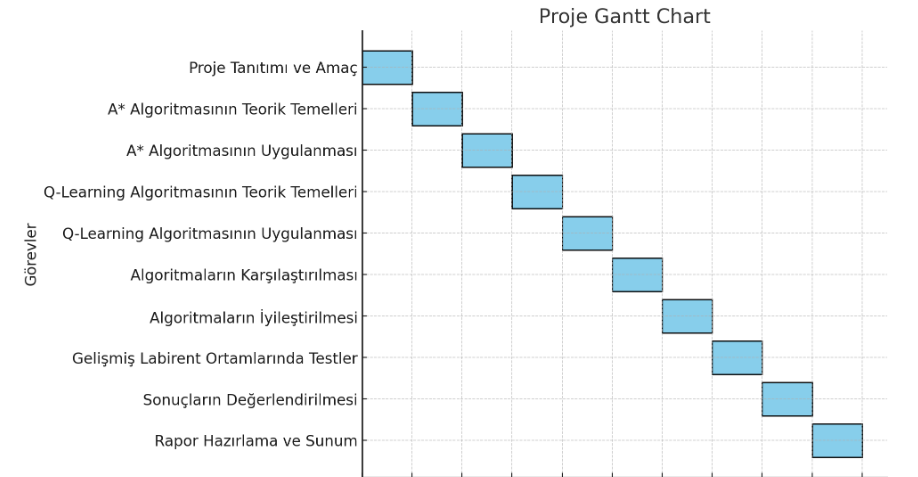
\includegraphics[height= 5 cm]{-gantt-chart.png}

		

			\end{figure}

	\end{landscape}	
	
	\section{Literatür Araştırması}	
	
a) Reinforcement Learning ile Çocuklarda Eğitsel Oyunların Geliştirilmesi:	Bu çalışmada, çocuklarda eğitsel oyunların geliştirilmesi için reinforcement learning (RL) yöntemlerinin kullanılması incelenmiştir. Eğitsel oyunlar, çocukların öğrenme süreçlerini desteklemek ve eğlenceli bir ortamda bilgi edinmelerini sağlamak amacıyla tasarlanmıştır. RL algoritmaları, bu oyunların içerisinde kullanılarak çocukların performansına göre oyunun zorluk seviyesinin dinamik olarak ayarlanması hedeflenmiştir. Örneğin, çocukların matematik becerilerini geliştiren bir oyun içerisinde, RL algoritmaları kullanılarak çocukların doğru cevaplar verme süreçleri analiz edilmiş ve oyunun zorluk seviyesi bu doğrultuda ayarlanmıştır.
b)Yapay Zeka Destekli Öğrenme Oyunları ve Öğrenci Motivasyonu:
Bu çalışma, yapay zeka (AI) destekli öğrenme oyunlarının öğrenci motivasyonunu artırmadaki etkisini araştırmaktadır. RL, öğrencilerin eğitim materyalleriyle etkileşime geçerek öğrenme süreçlerini optimize etmeye yardımcı olabilir. Örneğin, bir dil öğrenme uygulamasında, RL algoritmaları kullanılarak öğrencilerin kelime dağarcığını artırmak için etkili stratejiler belirlenmiştir. Bu stratejiler, öğrencilerin başarım düzeyine göre dinamik olarak ayarlanarak öğrenme sürecinin kişiselleştirilmesi sağlanmıştır. Bu çalışma, AI destekli öğrenme oyunlarının öğrenciler üzerindeki motivasyonu ve öğrenme performansı üzerindeki etkilerini değerlendirerek, gelecekteki eğitim teknolojilerinin tasarımında rehberlik edebilir.
c) Robotik Eğitiminde Güçlendirme Öğrenme Yaklaşımı:
Bu araştırma, robotik eğitiminde güçlendirme öğrenme yaklaşımının etkisini incelemektedir. RL, robotların çevreleriyle etkileşime girerek yeni beceriler öğrenmelerini sağlayabilir. Örneğin, bir robotun belirli bir görevi gerçekleştirmesi için gerekli olan hareket dizilerini öğrenmesi için RL algoritmaları kullanılabilir. Bu çalışma, robotik eğitimde RL'nin kullanımının, öğrencilerin problem çözme becerilerini geliştirmede ve karmaşık görevleri yerine getirmede nasıl yardımcı olabileceğini araştırmaktadır. Bu bağlamda, robotik eğitiminde RL'nin potansiyel avantajları ve sınırlamaları değerlendirilmekted   Literatürde DPO(Derin pekiştirmeli öğrenme) ve robot navigasyonu ile ilgili birçok çalışma bulunmaktadır.Mnih et al. (2015), Nature dergisinde yayınlanan bir çalışmada, DPO kullanarak Atari oyunlarında insanüstü performans elde etmeyi başarmıştır. Bu çalışma, DPO'nun karmaşık ve dinamik ortamlarda öğrenme yeteneğini göstermesi açısından önemlidir.         Lillicrap et al. (2015): arXiv preprint arXiv:1509.02971'de yayınlanan bir çalışmada, DPO kullanarak robotik bir kolun sürekli kontrolünü sağlamıştır ."Derin Deterministik Politika Gradyanları (DDPG)" adı verilen bir DPO algoritması kullanarak robotik bir kolun sürekli kontrolünü sağlamıştır. Bu çalışma, DPO'nun karmaşık ve dinamik ortamlarda robotları kontrol etmek için kullanılabileceğini göstermesi açısından oldukça önemlidir.DDPG algoritması, robotik bir kolun eklem açılarını girdi olarak alıp, her bir eylemin (eklem torkları) beklenen ödülünü tahmin eden bir sinir ağı modeli oluşturmak için eğitilmiştir[3].  OpenAI Five (2019): Dota 2 oyununda insanları yenebilen bir DPO modeli geliştirmiştir. Bu proje, literatürdeki mevcut çalışmalardan farklı olarak, 3D bir labirent ortamında robot navigasyonu için DPO'yu kullanmaktadır. Ayrıca, projede kullanılan veri seti ve algoritmalar, robotun labirentte daha hızlı ve daha verimli bir şekilde gezinmesine imkan sağlamaktadır [4].

\begin{landscape}
	\begin{figure}[!ht]		
		\caption[]{}
		\centering
		
		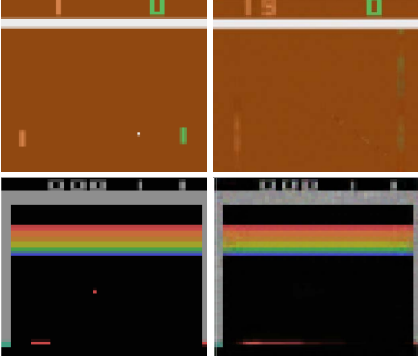
\includegraphics[height= 5 cm]{atarioyun.png}
		\label{}	
		
		\caption[]{}
		\centering
		
		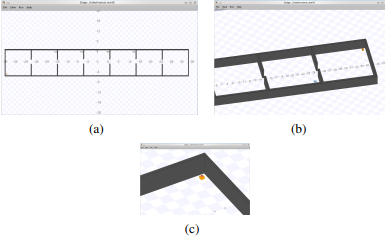
\includegraphics[height= 5 cm]{robotoyun.png}
		\label{}	
		\caption[]{}
		\centering
				
		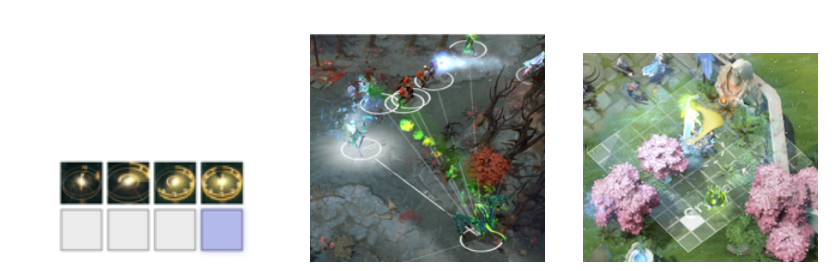
\includegraphics[height= 5 cm]{dota2.png}
		\label{}	
		
		

	\end{figure}
\end{landscape}	



	
	\section{Metodoloji} 
\begin{landscape} 
	\begin{itemize}
\item	İki nokta arasındaki tahmini maliyeti hesaplar (Manhattan mesafesi kullanılır).Manhattan mesafesi, iki nokta arasındaki yatay ve dikey mesafelerin toplamını ifade eder.Özellikle bir noktadan diğerine doğrudan gidilemeyen durumlarda,iki nokta arasındaki en kısa yolu tahmin etmek için kullanılır.Bu mesafe, yatay ve dikey yönlü hareketlerin toplamıdır,yani bir noktadan diğerine gitmek için sadece yatay ve dikey hareketlere izin verilir.Manhattan mesafesi, adını New York şehrinin sokak düzeninden alır;çünkü Manhattan semtinde sokaklar çoğunlukla dikdörtgen bir ızgara şeklinde düzenlenmiştir.Bu mesafe hesaplaması, genellikle yol bulma algoritmalarında, grafiklerde ve diğer birçok uygulamada kullanılır.		
	
\end{itemize}
	\begin{figure}[!ht]		
		\caption[]{}
		\centering
		
		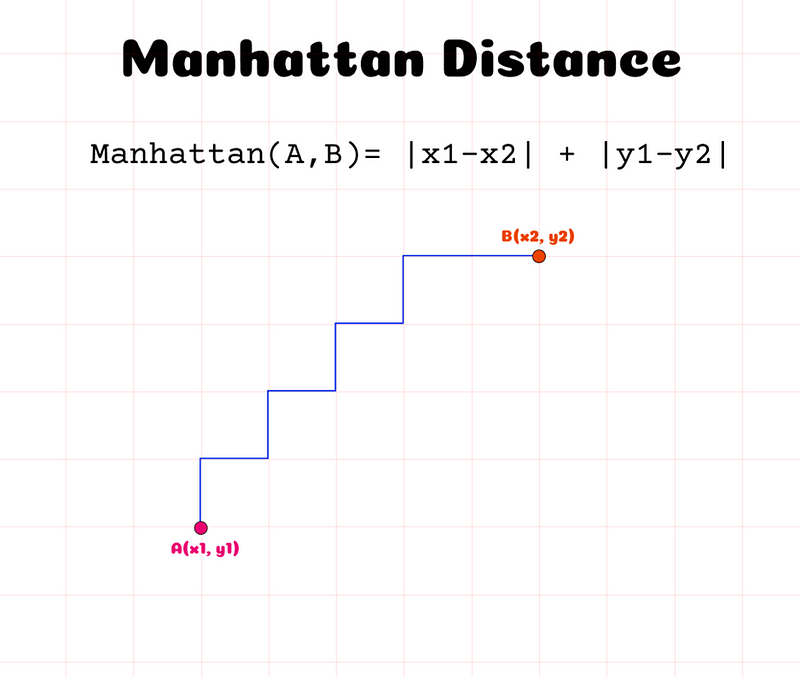
\includegraphics[height= 5 cm]{manhattan.png}

		\label{}	

		
	\end{figure}
\end{landscape}	



\begin{landscape}
	\begin{figure}[!ht]		
		\caption[]{}
		\centering
			
		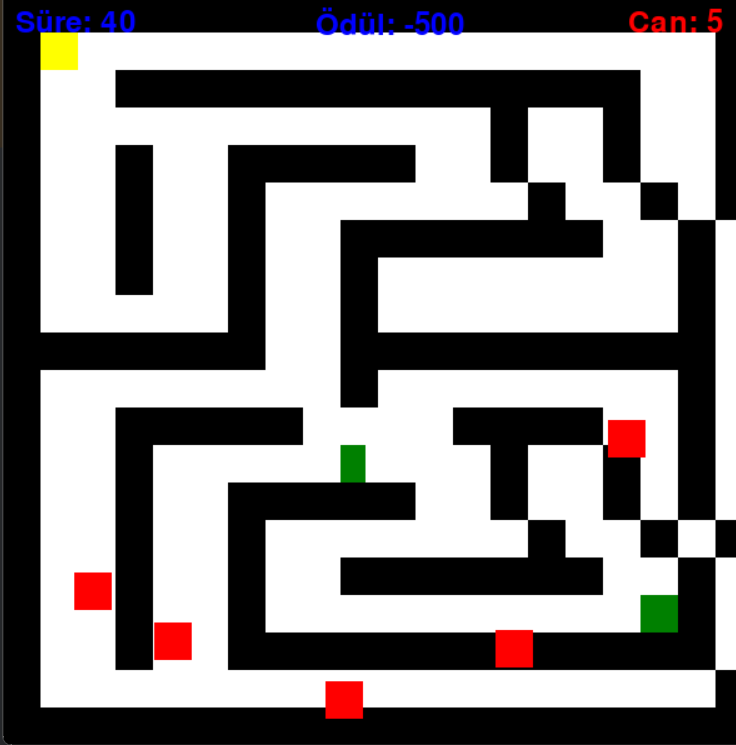
\includegraphics[height= 5 cm]{son.png}
		\label{}	
			
		
	\end{figure}
\end{landscape}	
	
\section {VeriTabanı ve Veriler :}%Sonuçlar-Tartışma

Reinforcement learning (RL), bir yapay zeka modelinin çevresiyle etkileşime 
geçerek deneyimlerden öğrenmesini sağlayan bir öğrenme paradigmasıdır.RL'nin temel amacı, bir ajanın belirli bir görevi en iyi şekilde nasıl gerçekleştireceğini öğrenmesidir. Bu öğrenme süreci, ajanın çevresiyle etkileşim halinde olması ve bu etkileşimlerden gelen geri bildirimlere dayanır.RL'de, ajan bir ortamda belirli bir görevi gerçekleştirirken karşılaştığı durumları ve bu durumlara verdiği tepkileri öğrenir. Ajan, bu durumlar ve tepkiler arasındaki ilişkileri anlayarak, belirli bir hedefe ulaşmak için en uygun eylemleri seçmeyi öğrenir. Bu süreçte, ajanın hedefe ulaşma performansı, aldığı ödüller veya cezalarla ölçülür. Amacı, bu ödül sinyallerini en üst düzeye çıkaran stratejileri öğrenerek belirli bir görevi en iyi şekilde gerçekleştirecek politikaları bulmaktır.Özetle, reinforcement learning'in amacı, bir yapay ajanın bir görevi en iyi şekilde gerçekleştirmesini sağlayacak stratejileri öğrenmesidir.Bu süreçte, ajan deneyimlerinden öğrenir ve çevresinden gelen geri bildirimleri kullanarak kendisini geliştirir.

	\begin{figure}[h]
	\centering		
	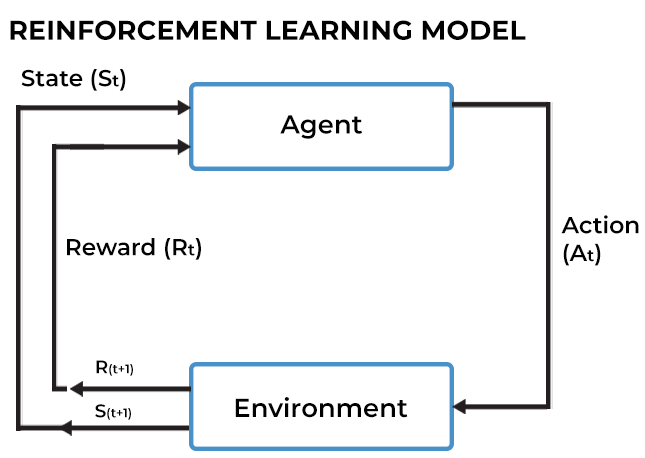
\includegraphics[height= 5 cm]{photo1-}		
	\label{}
\end{figure} 
\centering 


	%Kaynakçayı yazdırmak
	
	\bibliography{ref.bib}
	\bibliographystyle{ieeetr}
	%\printbibliography %Prints bibliography
	
	\cite{berner2019dota}.
	\cite{gokcce2013implementation}.
	\cite{aydin2020using}.
	\cite{openai_chatgpt}
	\cite{gullu2017labirentlerde}.
	\cite{boluk2019mobil}.
	\cite{kavasougluyapay}.

		
	
	\input{}
	



\end{document}
